\begin{table}[htb]
  \centering
  \caption{Resource usage by entity, including resources used by sub-entities.}
  \begin{tabular}{llll}
    \toprule
                         & LC Combinationals & LC Registers & Memory Bits \\
    \midrule
    Fetch Stage          & 61                & 14           & 131072      \\
    Decode Stage         & 1659              & 1080         & 0           \\
    -- Register File     & 1085              & 1034         & 0           \\
    Execute Stage        & 1206              & 172          & 0           \\
    -- ALU               & 444               & 0            & 0           \\
    Memory Stage         & 186               & 115          & 0           \\
    -- Jump Unit         & 4                 & 0            & 0           \\
    -- Memory Unit       & 59                & 0            & 0           \\
    Write-Back Stage     & 110               & 38           & 0           \\
    Forwarding Unit      & 20                & 0            & 0           \\
    Control Unit         & 301               & 225          & 0           \\
    \cmidrule{1-4}
    Sum                  & 3325              & 1644         & 131072      \\
    \bottomrule
  \end{tabular}
\end{table}

\begin{qa}
  \question{What is the maximum frequency of your design?}
  \answer{86.89 MHz}
  \question{Where is the critical path of your design?}
  \answer{from regfile: rdaddr2\_reg to ctrl: npc}
\end{qa}

\begin{figure}[ht!]
\centering
\framebox[\linewidth]{
%\rotatebox{30}{Insert your figure here.}
}
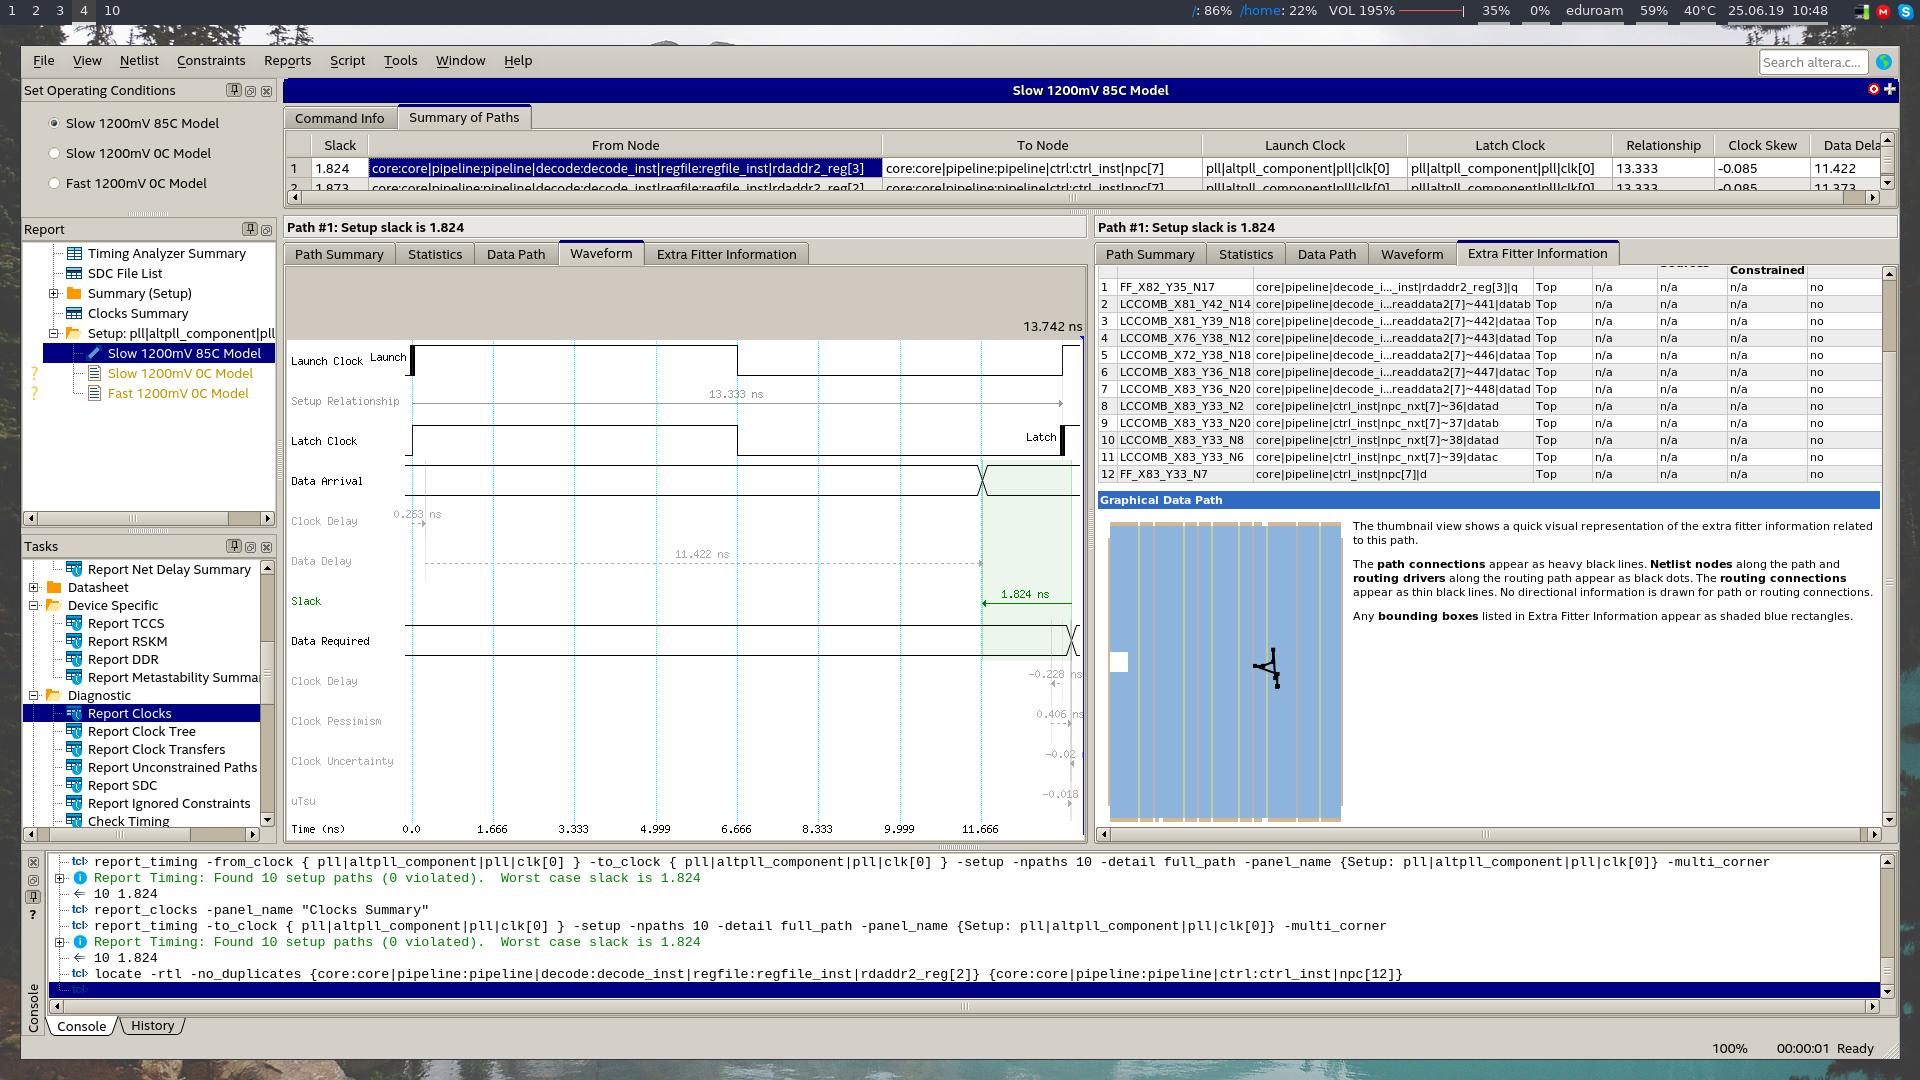
\includegraphics[width=1.0\linewidth]{task3.jpg}
\caption{Simulation screenshot for critical path.}
\end{figure}
